\setchapterstyle{kao}
\setchapterpreamble[u]{\margintoc}
\chapter{Turbo Rascal Syntax}
\labch{intro}

\section{Introcuction}

\begin{minipage}{0.2\textwidth}
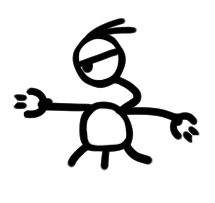
\includegraphics[width=\linewidth]{images/trip/trip2.png}
\end{minipage}
\begin{minipage}{0.8\textwidth}\raggedleft
The programming language used in TRSE is called "Rascal" for a good reason. Developed as a practical hybrid language, it is a mix of 80\% Pascal with 20\% C standards, whichever suited the developer at the time of creation. Therefore, Turbo Rascal can not be considered a fully Pascal-compliant language, since it contains some quirks. That being said, most of the syntax is definitely very Pascal-compliant indeed.   
\end{minipage}
\subsection{Program structure}
\begin{lstlisting}
Program MyProgram;
var
    a,b,c : byte = 0;
 
Procedure Myprocedure(mp_i:byte);
var
  somProcedureVariable : byte;
begin
  // Do someting
end;
 
// This is the main block.
begin
   // Call user-defined procedures etc
   MyProcedure(2);
end.
\end{lstlisting}
\subsection{Supported types}
TRSE supports several data types:
\begin{itemize}
  \item byte : values 0-255
   \item integer: values 0-65535
  \item pointer : 16 address
  \item strings are stream of bytes that are terminated with "0"
  \item incbin : include binary file
  \item incsid : include SID file
\end{itemize}
The motorola 68000 as some additional types:
\begin{itemize}
    \item long : 32 bit numbers
    \item pointer of byte/integer/long : pointer to byte/integer/long array (motorola 68000 only)
    \item chipmem specifier: myArray: array[255] of byte chipmem
\end{itemize}
Declaration examples:
\begin{lstlisting}
var
   a,b,c : byte; // will default be "0"
   d,e,f : byte = $5; // initialized with value $5
   g : integer = $1000;
   text : string = ("A STRING", 34, " CAN CONSIST OF BOTH", 45, 99, "TEXT AND NUMBERS"); // terminated by "0"
   data : incbin("data/myTable.bin", $2000); // Include data file at memory position $2000
   zp, cp : pointer; // zeropage pointers that can point to other variables / arrays
\end{lstlisting}
\subsection{Arrays}
Arrays are defined in the following manner:
\begin{lstlisting}
@define someConstant 25
 
var
   myArray1 : array[128] of byte; // 128 bytes of zeros are declared
   myArray2 : array[4*3] of byte = (0,5,$90, @someConstant);
   myArray3 : array[] of integer = ($1000, $2000, $3000); // unspecified array count
   myArray4 : array[255-55] of byte = (1,2,3); // only 3 values defined, rest will be padded with zeros.
\end{lstlisting}
Arrays that have no intialization values are filled with "0" by default. 
Arrays (both integer and bytes) are accessed as such:
\begin{lstlisting}
myArray[i]:=someValue*5;
\end{lstlisting}
There is no out-of bonds testing in TRSE.
\subsection{Conditionals}
An if-else block in TRSE is defined as such:
\subsubsection{If}
\begin{lstlisting}
if (a=1) then DoSomething();
if (a<>3) then 
begin
   DoSomethingElse();
   IgnoreMe(4);
end;
if (a*2=b*3) then 
   return() 
else
  somethingelse()
\end{lstlisting}
Do not the missing ";" before an else-block. This is a typical symptom of Pascal. 
A final note: The “empty” conditional
\begin{lstlisting}
if (a) then DoSomething() else DoSomethingElse();
\end{lstlisting}
is the same as typing “if (a<>0)” or "if (a<>true)" (if a is not true).
\subsubsection{While}
While conditionals works similar to if statements:
\begin{lstlisting}
while (a>0) then do 
begin
  PrintSomething(a);
  dec(a);
end;
\end{lstlisting}

\subsubsection{Case}
Cases tests a single variable for multiple values as such:
\begin{lstlisting}
 case i of:
   0: DoSomething();
   1: begin 
        HelloThere();
        b:=b+5;
      end;
   2+i : ThisIsWeird();
  else 
     begin
       PerformElseBlock();
     end;
\end{lstlisting}
The else block is optional.

\subsection{For loops}
For 6502 systems, only bytes are allowed as counter variables, restricting the counting loop to 256 iterations. 
\begin{lstlisting}
for i:=0 to 10 do 
begin
   doSomething(i);
end;
 
for j:=a to b step 2 do 
  someArray[j]:=a+b*j;

for j:=0 to 256 do myTable[j]:=j/16; // same as for j:=0 to 0 do ...
\end{lstlisting}
In order to overcome the 256 byte limitations, zero page pointers should be used. For instance, in order to fill the entire screen memoru at \$0400 with data, we use the following nested loop:
\begin{lstlisting}
program fillScreenWithRandomValues;
var
  x,y : byte;
  zp : pointer;

begin
	// Repeat for ever
	while (true) do
	begin

		zp:=screen_char_loc; 
		// zp now points to the screen character location (at $0400)

		// Now loop through 25 rows on the screen
		for y:=0 to 25 do 
		begin
			for x:=0 to 40 do
				zp[x]:=Random(); //Set the character with some random value

			// Increase the screen pointer by 40 bytes (width of screen)
			zp:=zp+40; 
		end;
	end;
end.
\end{lstlisting}


\subsection{Procedures}
Procedures are defined as such:
\begin{lstlisting}
Procedure NoParameters();
begin
   // .. code here
end;
 
// Procedure with single parameter and variable block
procedure DoSomething(a,b:byte; zp: pointer);
var
  localVar : byte;
 
begin
   zp:=zp+a;
   localVar := a+b; 
   // ...
end;

\end{lstlisting}
You can return byte values from procedures by using the ReturnByte(value) method. 
\begin{lstlisting}
Procedure CalculateSomeStuff(v:byte);
begin
	ReturnByte(v*2 +1);
end;

...

begin
	a:=CalculateSomeStuff(i/3)*5-1;

...
\end{lstlisting}

\subsection{Preprocessors}

\subsubsection{Constants}
\begin{lstlisting}

\end{lstlisting}

\subsubsection{Ifdef/ifndef}
\begin{lstlisting}

\end{lstlisting}
